\section{Contextualização}

\begin{frame}
	\begin{block}{Contextualização}
		\begin{enumerate}
			\item Classificadores definem uma superfície de decisão para classificar dados (em até n-classes)
		\end{enumerate}
		\begin{figure}[!htb]
			\centering	  				
			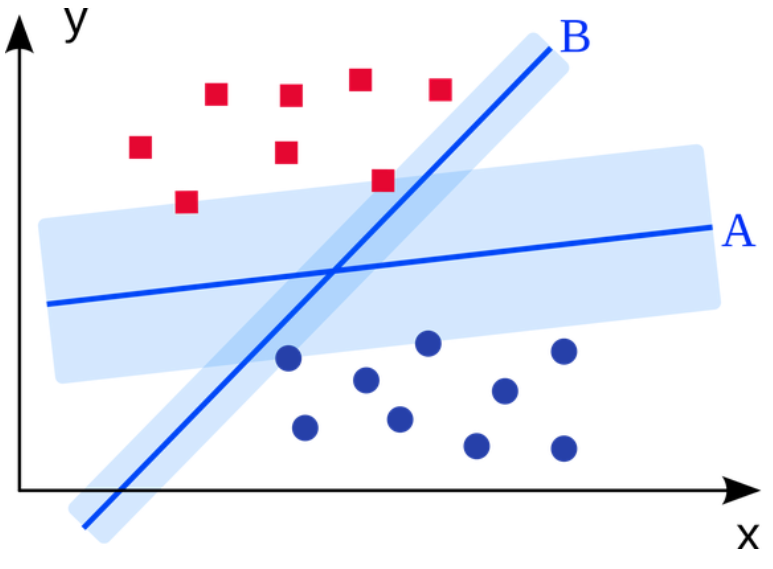
\includegraphics[height=4cm, width = 7cm]{./pic/fronteirautopia.png}
			\caption{Exemplo utópico de fronteira de decisão}
			\label{fig_ds_process}
		\end{figure}	
	\end{block}
\end{frame}

\begin{frame}
	\begin{block}{Contextualização}
		\begin{enumerate}
			\item Os classificadores escolhem uma das retas azuis possíveis (há infinitas possibilidades) para ser a fronteira de decisão.
			\item O problema acima é utópico, tipicamente as classes não ficam separadas perfeitamente.
		\end{enumerate}
			\begin{figure}[!htb]
			\centering	  				
			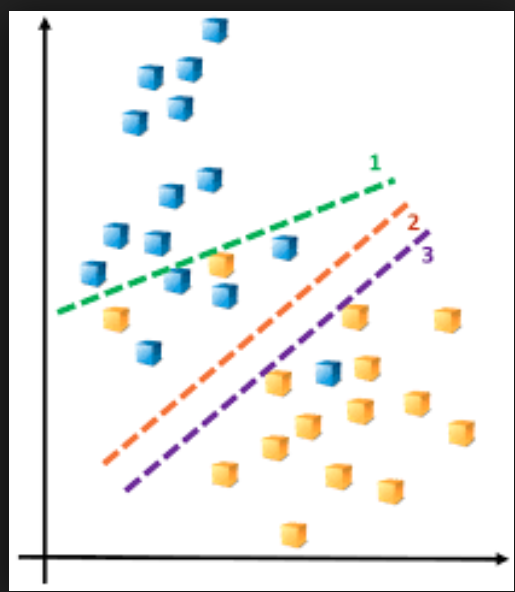
\includegraphics[height=4cm, width = 7cm]{./pic/fronteirareal.png}
			\caption{Exemplo real de fronteira de decisão}
			\label{fig_ds_process}
		\end{figure}	
	\end{block}
\end{frame}

\begin{frame}
	\begin{block}{Contextualização}
		\begin{enumerate}
			\item Para definir a fronteira é usado um algoritmo de otimização (que minimiza o erro de classificação)
			\item \textbf{É considerado normal ter erros de classificação dado a natureza não determinística dos algoritmos de Machine Learning}
		\end{enumerate}
	\end{block}
\end{frame}

\begin{frame}
	\begin{block}{Contextualização}
	Quando ocorre um erro de classificação em algoritmos de machine learning podem ter várias razões (não mutuamente exclusivas):
		\begin{enumerate}
					\item Dados de treino insuficientes/viesados
					\item Arquitetura do algoritmo mal planejada
					\item O algoritmo aprendeu a função errada
					\item Bug no código fonte
					\item Variação na distribuição das principais variáveis usadas pelo modelo
					\item Bug em outros sistemas que alimentam os dados do modelo
		\end{enumerate}
	\end{block}
\end{frame}



\begin{frame}
	\begin{block}{Contextualização}
		\begin{enumerate}
			\item Além dos problemas citados há modelos caixa preta (não é possível entender como o modelo toma decisões[de onde foi criado o score?])
			\item Regressão logística e CART são exemplos de algoritmos interpretáveis (é possível entender como foi tomada a decisão)
		\end{enumerate}
	\end{block}
\end{frame}



\begin{frame}
	\begin{block}{Contextualização}
		\begin{enumerate}
			\item Dados todos esses problemas citados há linhas de pesquisa para cada um deles.
			\item Os artigos LIME, SHAP e manifold tentam resolver o problema de quais variáveis são mais relevantes para modelos caixa preta.
			\item O último artigo trata sobre identificação de bugs em código fonte de algoritmos de Machine Learning
		\end{enumerate}
	\end{block}
\end{frame}

